\begin{frame}{Contexto}
  \renewcommand{\arraystretch}{1.8} % Espaciado vertical entre filas (opcional)

  \begin{tabular}{ >{\raggedright\arraybackslash}m{0.6\linewidth} >{\centering\arraybackslash}m{0.35\linewidth} }
    \begin{itemize}
      \item Intrusiones en sistemas informáticos.
    \end{itemize} &
    
\includegraphics[width=\linewidth]{./img/ciberia.png} \\
    
    \begin{itemize}
      \item Evolución de los ataques a las redes informáticas como consecuencia del uso de IA.
    \end{itemize} &
    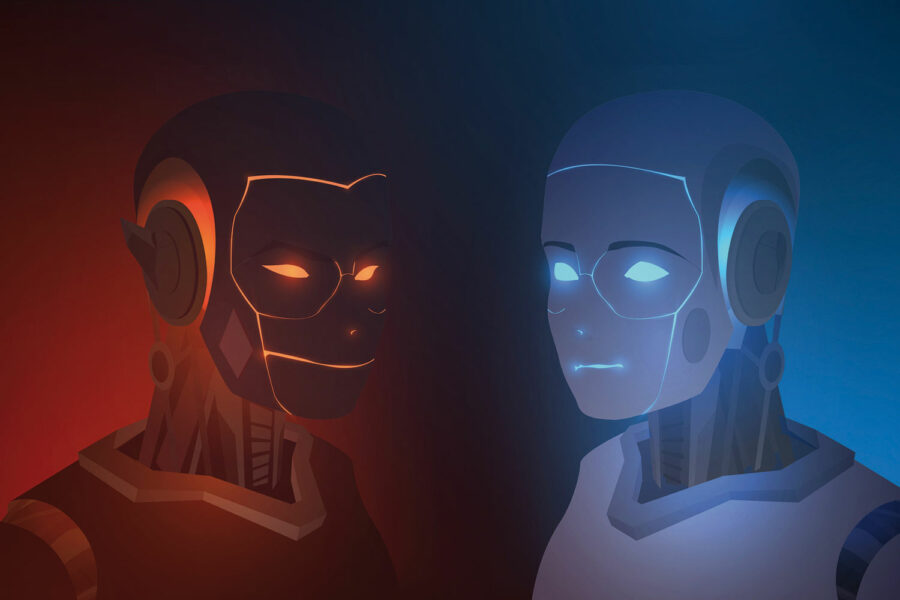
\includegraphics[width=\linewidth]{./img/iavsia.png} \\

    \begin{itemize}
      \item Defensa ante posibles intrusiones.
    \end{itemize} &
    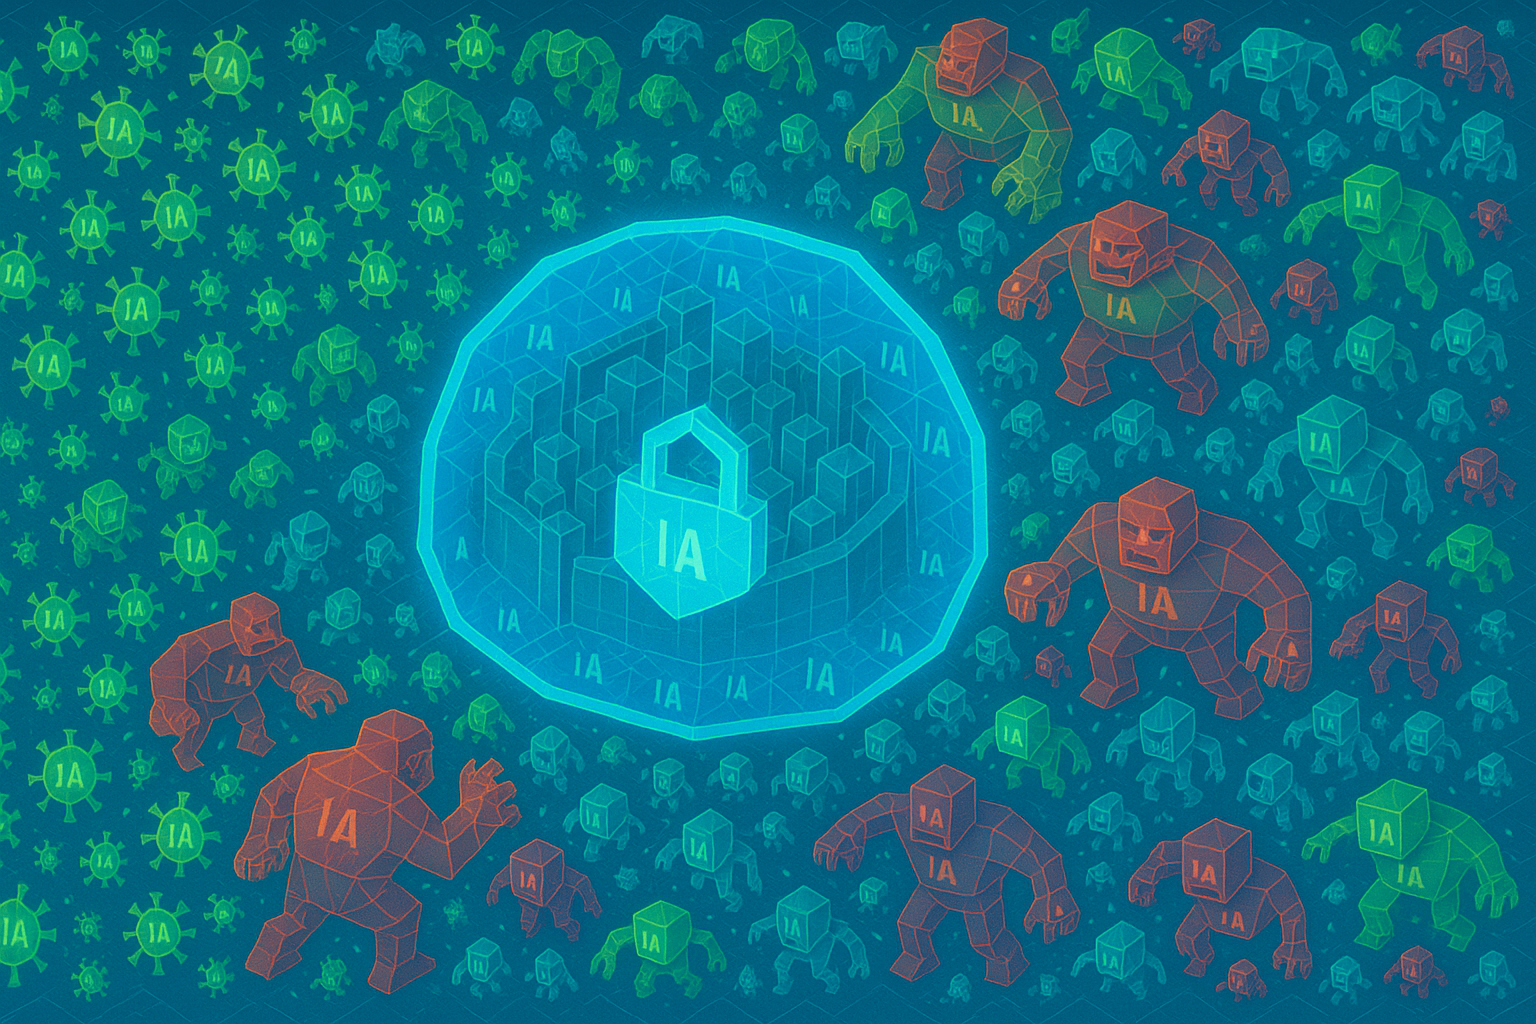
\includegraphics[width=\linewidth]{./img/atacados.png} \\
  \end{tabular}
\end{frame}


\begin{frame}{Objetivos del proyecto}
    \begin{enumerate}
        \item  Diseñar e implementar un modelo capaz de detectar intrusiones en redes informáticas y proporcionar una clasificación previa de la intrusión.
        \vspace{10mm}
        \item Desarrollar modelos de detección que han de ser modelos neuronales.
        \vspace{10mm}
        \item Evaluar y comparar los modelos generados con un \textit{dataset} real y complejo.
    \end{enumerate}
\end{frame}

%\begin{frame}{Objetivos del académicos}
%    \begin{itemize}
%        \item Comprender el funcionamiento de los modelos neuronales a través de PyTorch y las métricas de evaluación.
%        \vspace{10mm}
%        \item Asimilar las características de varios tipos de modelos neuronales existentes.
%        \vspace{10mm}
%        \item Descubrir el potencial de las redes neuronales para optimizar y mejorar las tecnologías de la información, incluyendo la ciberseguridad de los sistemas.
%        \end{itemize}
%\end{frame}